%%
%% $Id$
%%
%% Copyright (c) 2007-2008 Christian Fehler
%% Copyright (c) 2007-2008 Benjamin Mies
%%


%### removes texlipse warnings


\chapter{Oberfläche}\label{GUI}

In diesem Kapitel geht es um die Oberflächengestaltung. Zum Einen geht es darum,
wie und warum die Hauptansicht so gestaltet wurde, zum Anderen darum, welche
besonderen Schritte notwendig waren, um das Aussehen zu verbessern und dem
Benutzer es dadurch zu erleichtern, mit dem \gtitool zu arbeiten.
\vspace{10pt}


\section{Gestaltung der Hauptansicht}\label{GUIMain}

Als wir zu Beginn der Diplomarbeit über die Gestaltung der Hauptansicht
diskutiert haben, kamen wir sehr schnell zu der Übereinkunft, dass die
Ähnlichkeit zu dem Lernwerkzeug TPML möglichst groß sein sollte. Da sowohl
"`Grundlagen der theoretischen Informatik"', als auch "`Theorie der
Programmierung I"' für jeden Informatikstudenten der Universität Siegen
Pflichtveranstaltungen sind, ist die Wahrscheinlichkeit, dass Studenten beide
Lernwerkzeuge nutzen werden, sehr hoch.\vspace{10pt}

Ein großer Vorteil dieser Entscheidung war natürlich, dass wir beide
bereits an der Projektgruppe TPML mitgearbeitet hatten. Zwar waren wir nicht
hauptsächlich an den Grafikelementen beteiligt, konnten aber dennoch einige
Einblicke sammeln, welche uns bei der Gestaltung der Benutzeroberfläche sehr
geholfen haben.\vspace{10pt}

Wir hoffen, dass zukünftige Benutzer von den Parallelen im Aussehen
und in der Funktionsweise beider Lernwerkzeuge profitieren können.\vspace{10pt}

Während der gesamten Diplomarbeit stand im Vordergrund, das Lernwerkzeug so
intuitiv und selbsterklärend wie möglich zu gestalten. Denn schließlich soll
ein Benutzer nicht noch lange Zeit darauf verwenden müssen, den Umgang mit dem
Werkzeug zu erlernen und sich im schlimmsten Falle durch ein dickes Handbuch
durchzuarbeiten.\vspace{10pt}

Aus diesem Ansatz heraus ist zum Beispiel auch der Wizard zum Anlegen einer
neuen Datei enstanden. Dieser Wizard hat für jedes Eingabefeld ja schon einen
Vorschlag, welche in den Einstellungen auf die Benutzerwünsche angepasst werden
kann. Beim ersten Start sollen diese Werte als Orientierung dienen, was in den
Feldern eingetragen werden soll.
\vspace{10pt}


\section{Gestaltung der graphischen Komponenten}\label{GUIDesign}

TODOCF: Navigations-Buttons
TODOBM: PrettyString
TODOBM: Tabelleneinträge highlighten



\section{Redo/Undo}\label{GUIRedoUndo}

Da das Lernwerkzeug vom Aussehen her sehr an einen Editor angelehnt ist,
wollten wir dem Benutzer auch eine Möglichkeit geben, Schritte rückgängig zu
machen oder zu wiederholen. Dies war jedoch zu einem Zeitpunkt, zu dem bei
weitem noch nicht alle Funktionalität implementiert war. Desweiteren soll das
Werkzeug ja auch zukünftig an den Stoff der Vorlesung angepasst werden, so dass
uns eine einfache Erweiterbarkeit sehr wichtig war.\vspace{10pt}

Daher haben wir uns entschlossen, die Verwaltung der Redo/Undo Schritte nicht
einer Klasse alleine zu überlassen, sondern die verschiedenen Aktionen in
einzelnen Items zu kapseln. Auf diesen Items kann dann die entsprechende Redo-
bzw. Undo-Funktion aufgerufen werden. Verwaltet wird dies von einem Handler,
welcher sich nur merkt, welches das letzte aktive Item für Redo und Undo ist,
und den Aufruf durch den Nutzer an das Item weiterleitet.\vspace{10pt}

Durch diese Kapselung ist es leicht möglich, die Redo/Undo Funktion zu
erweitern, da einfach ein neues Item für die entsprechende Aktion implementiert
werden muss, um diese Item beim Ausführen der Aktion an den Handler zu
übergeben.\vspace{10pt}


\section{Anpassung aller GUI Komponenten}\label{GUIAdaption}

Ein wichtiges Konzept bei der graphischen Gestaltung des \gtitool ist es, die von
der Programmiersprache zur Verfügung gestellten Komponenten anzupassen und dann
nur noch ausschließlich diese angepassten Komponenten zu benutzen. Der Vorteil
dieser Umsetzung ist, dass nicht überall ein normaler String verwendet wird,
sondern ein sogenannter Pretty-String. Dieser enthält neben dem eigentlichen
Text auch noch Farbinformationen, sowie Zeichenattribute, wie zum Beispiel
Fettdruck.\vspace{10pt}

Der erforderliche Aufwand wurde investiert, um dem Benutzer eine möglichst
ansprechende Oberfläche zu präsentieren und ihn durch die zusätzlichen
Informationen zu unterstützen, die Inhalte besser zu verstehen.\vspace{10pt}

Ein weiterer wichtiger Ansatz war, dass der Benutzer das \gtitool möglichst
intuitiv bedienen kann. Zur Umsetzung wurde unter anderem Drag and Drop auf den
verschiedenen Komponenten implementiert. So kann der Benutzer im Übergangs-Dialog
die Symbole einfach vom "`Alphabet"' in die "`Übergangs-Menge"' ziehen. Gleiches
gilt für das Umsortieren von Produktionen, wodurch zwar die Grammatik nicht
geändert wird, es dem Benutzer aber möglich ist, die Produktionen übersichtlicher
anzuordnen. In vielen Programmen, in denen Tabs zur Gliederung benutzt werden,
gehört es zum Funktionsumfang diese Tabs per Drag and Drop zu verschieben. Auch
dies wurde implementiert, da es dem Benutzer erlaubt, seine Daten besser zu
organisieren.\vspace{10pt}


\section{Look \& Feel}\label{LookAndFeel}

Damit das \gtitool unter verschiedenen Betriebsystemen immer gleich, oder
zumindest sehr ähnlich aussieht, kam während der Entwicklung der Wunsch auf, ein
eigenes Look \& Feel zu verwenden. Java bietet in diesem Bereich zwar mit dem
Metal Look \& Feel eine Lösung an, die unter allen Betriebssystemen gleich
aussehen soll, diese erfüllte aber unsere Vorstellungen nicht. Schließlich fiel
die Wahl auf TinyLaF (siehe \cite{tinylaf}), ein weitgehend gezeichnetes
Look \& Feel, dass somit unter allen Betriebsystemen gleich aussieht. Dem
Benutzer ist es aber freigestellt, ein anderes, zum Beispiel das normale
Betriebsystem Look \& Feel zu verwenden, wenn er dies wünscht. Alle in dieser
Diplomarbeit verwendeten Bilder des \gtitools wurden mit TinyLaF als Look \&
Feel gemacht.\vspace{10pt}


\section{Zweite Ansicht}\label{SecondView}

Bei der Umsetzung der verschiedenen Algorithmen wurden wir vor das Problem
gestellt, dass es sinnvoll wäre, einen Automaten nach der Umwandlung, mit dem
Automaten oder der Grammatik vor der Umwandlung zu vergleichen. Dies war nur
durch einen Tabwechsel oder das Öffnen eines zweiten \gtitools möglich, was
nicht besonders benutzerfreundlich ist.\vspace{10pt}

\begin{figure}[h!]
\begin{center}
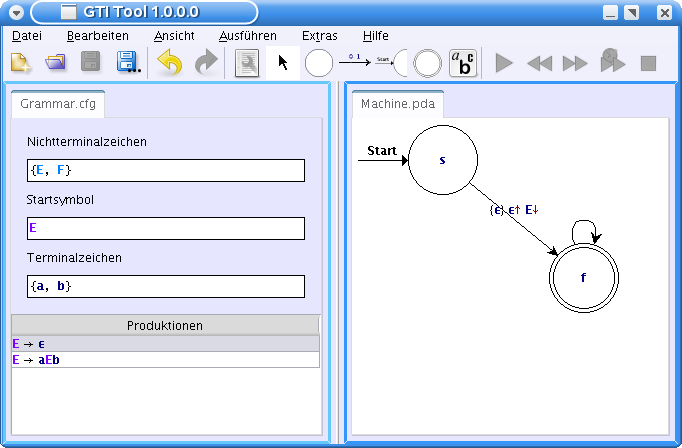
\includegraphics[width=12cm]{../images/second_view.png}
\caption{Zweite Ansicht}
\label{FigureSecondView}
\end{center}
\end{figure}
\vspace{10pt}

Dieses Problem wurde dadurch gelöst, dass eine zweite Ansicht integriert wurde,
die es erlaubt, Tabs in einem zweiten Bereich zu öffnen. So können zwei Dateien
gleichzeitig sichtbar sein. Während der Umsetzung mussten verschiedene Probleme
diskutiert und gelöst werden. So stellte sich die Frage, wie dem Benutzer
verdeutlicht werden kann, welche der beiden sichtbaren Dateien aktiv ist. Wichtig
ist dieser Status für die Aktivierung der Menüeinträge bzw. Toolbar Buttons. Als
Umsetzung wurde schließlich gewählt, dass anhand von unterschiedlichen
Umrandungen dem Benutzer klar gemacht werden soll, welche der beiden Dateien die
aktive ist. Durch dieses Vorgehen wird intuitiv klar, welche Datei aktiv ist, da
sich die Farbe der Umrandung beim Aktivieren der anderen Ansicht ändert. In
Abbildung \ref{FigureSecondView} ist der Automat auf der rechten Seite
aktiv.\vspace{10pt}

Eine weitere wichtige Eigenschaft der zweiten Ansicht ist, dass Dateien in diese
zweite Ansicht verschoben werden können. Ebenfalls muss es möglich sein in der
zweiten Ansicht Dateien zu öffnen bzw. neue zu erstellen. Um die letzen beiden
genannten Punkte umzusetzen, wurde das Konzept des aktiven Editors erweitert. Die
oben beschriebene andere Darstellung der aktiven Datei wurde so erweitert, dass
sich auch alle anderen Ereignisse auf den aktiven Editor beziehen. Wenn eine
Datei geöfffnet werden soll, muss erst die Ansicht aktiviert werden, in der die
Datei geöffnet werden soll. Das Gleiche gilt beim Anlegen einer neuen Datei. Das
Verschieben von geöffneten Dateien wurde per Kontextmenü und intuitiv per Drag
and Drop zwischen den Ansichten gelöst.\vspace{10pt}


%### removes texlipse warnings
